\documentclass[10pt,a4paper]{article}
\usepackage[utf8]{inputenc}
\usepackage[russian]{babel}
\usepackage[OT1]{fontenc}
\usepackage{amsmath}
\usepackage{amsfonts}
\usepackage{amssymb}
\usepackage{graphicx}
\DeclareGraphicsExtensions{.pdf,.png,.jpg}
\usepackage[left=2cm,right=2cm,top=2cm,bottom=2cm]{geometry}

\begin{document}
\begin{equation}
y = \int_0^\infty \frac{e^{-z}}{(1 + x z)}\;\mathrm{d}z = \frac{e^{1/x} \Gamma \left(0,\frac{1}{x}\right)}{x},\Im(x)\neq 0\lor \Re(x)\geq 0
\end{equation}
Как видно из графиков максимальное значение интеграла $\approx$ 2 и достигается при $x\approx 0.001354$\\
При $x<0.001354$ значение интеграла 0\\
При $x>0.001354$ значение будет "осциллировать" с убывающей амплитудой, а "среднее" будет просто убывать, стремясь к 0 
\begin{figure}[h]
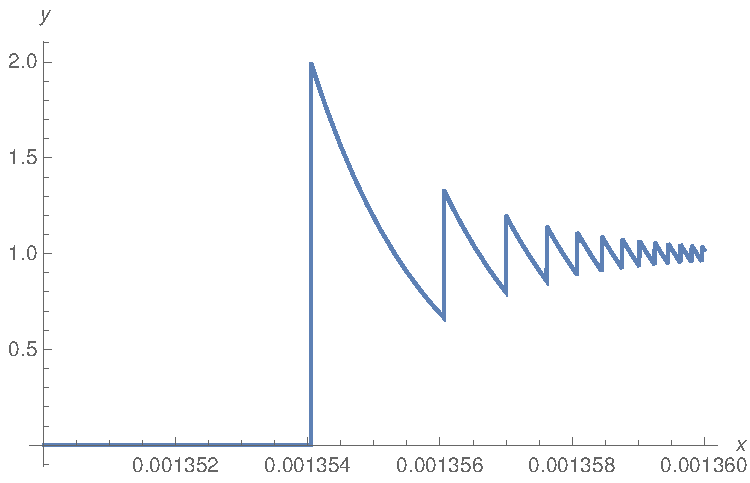
\includegraphics{gr1}
\end{figure}

\begin{figure}[h]
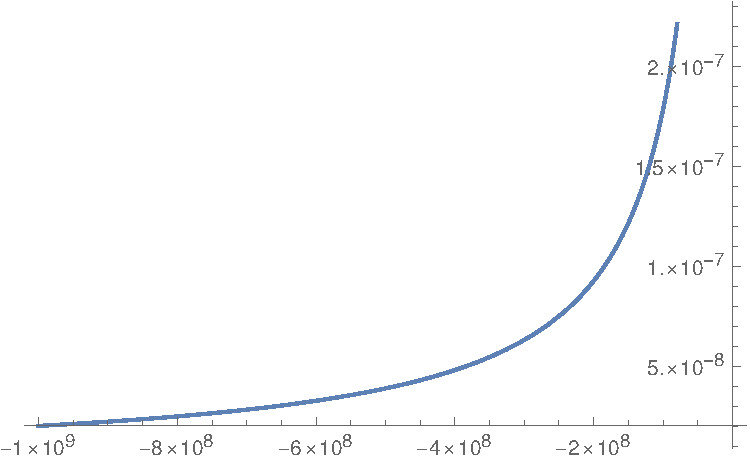
\includegraphics{gr2}
\end{figure}

\begin{equation}
y_2 = \int_{-\infty }^{\infty } e^{-x z^4-\frac{z^2}{2}} \, dz = \frac{e^{\frac{1}{32 x}} K_{\frac{1}{4}}\left(\frac{1}{32 x}\right)}{2 \sqrt{2} \sqrt{x}},\Re(x)>0
\end{equation} 

Как видно из графиков максимальное значение интеграла $\approx$ 5.3 при $x\approx 0.0000421$\\
При $x<0.0000421$ значения максимума значение интеграла равно 0\\
При $x>0.0000421$ значения максимума значение интеграла начинает "осциллировать", а "среднее" будет убывать, стремясь к 0

\begin{figure}[h]
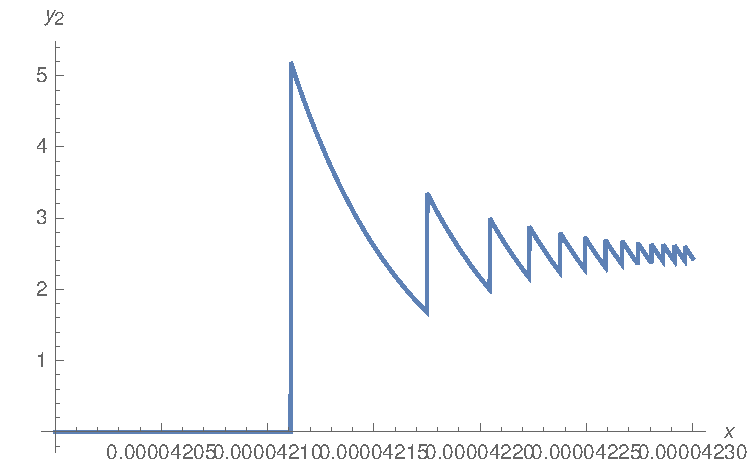
\includegraphics{gr4}
\end{figure}

\begin{figure}[h]
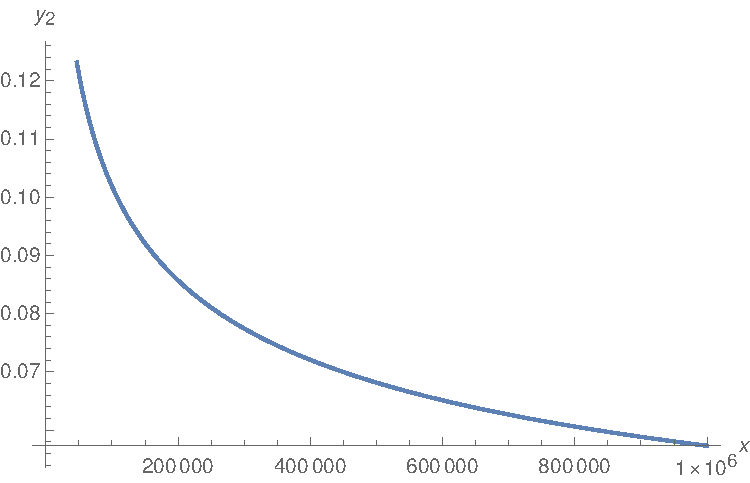
\includegraphics{gr5}
\end{figure}
\end{document}